\section{Achievements of Deep Learning}
Deep Learning has had an explosion in applications and research and development
for the last decade. These applications include:

\begin{itemize}
    \item Automatic speech recognition
    \item Image recognition
    \item Visual art processing
    \item Natural language processing
    \item Drug discovery and toxicology
    \item Customer relationship management
    \item Recommendation systems
    \item Bioinformatics
\end{itemize}

The theoretical foundations of the field is old (mid 19th century), but the 
playground for these algorithms has just now arrived. These include large
datasets, computational hardware and software. 

\section{Comparison with traditional machine learning}
In traditional machine learning development. One needs domain knowledge for
developing good models. Domain knowledge let's you select good features 
and good features give good models. One example could be a certain visual
feature in a certain kind of biomedical image. This field is called 
\textbf{feature engineering}. 

\section{Feature Learning}
Feature Learning, also known as \textbf{Representation Learning} is a set of
techniques that allow systems to automatically discover the representation 
needed for feature detection or classification. Feature learning methods 
let us replace the manual feature engineering that is done in traditional 
machine learning development. A lot of deep learning architectures for 
representation learning have been researched and published in the last decade.

\section{Motivations for deep learning}

Deep Learning let's us model nonlinear decision boundaries by introducing
nonlinearities in the activation functions and deep architectures. This means 
that deep learning is especially fit for problems that are too complex for 
linear methods. One could question wether models like logistic regression could
be used with polynomial decision boundaries to achieve the same thing. 
The problem with using regression is that it achieves this by introducing
polynomial features. The number of features the model must take into account
is then 

\begin{equation*}
    O(n^b)
\end{equation*}

where $b$ is the polynomial degree that you want the model to incorporate. 
For $100$ features, introducing $b = 2$ gives over 5000 features. This is not
feasible. 

\section{Artificial Neuron}
\begin{itemize}
    \item Feed input via input nodes
    \item Logistic unit does some computation
    \item Sends output
\end{itemize}

\bigskip
\begin{figure}[H]
\centering
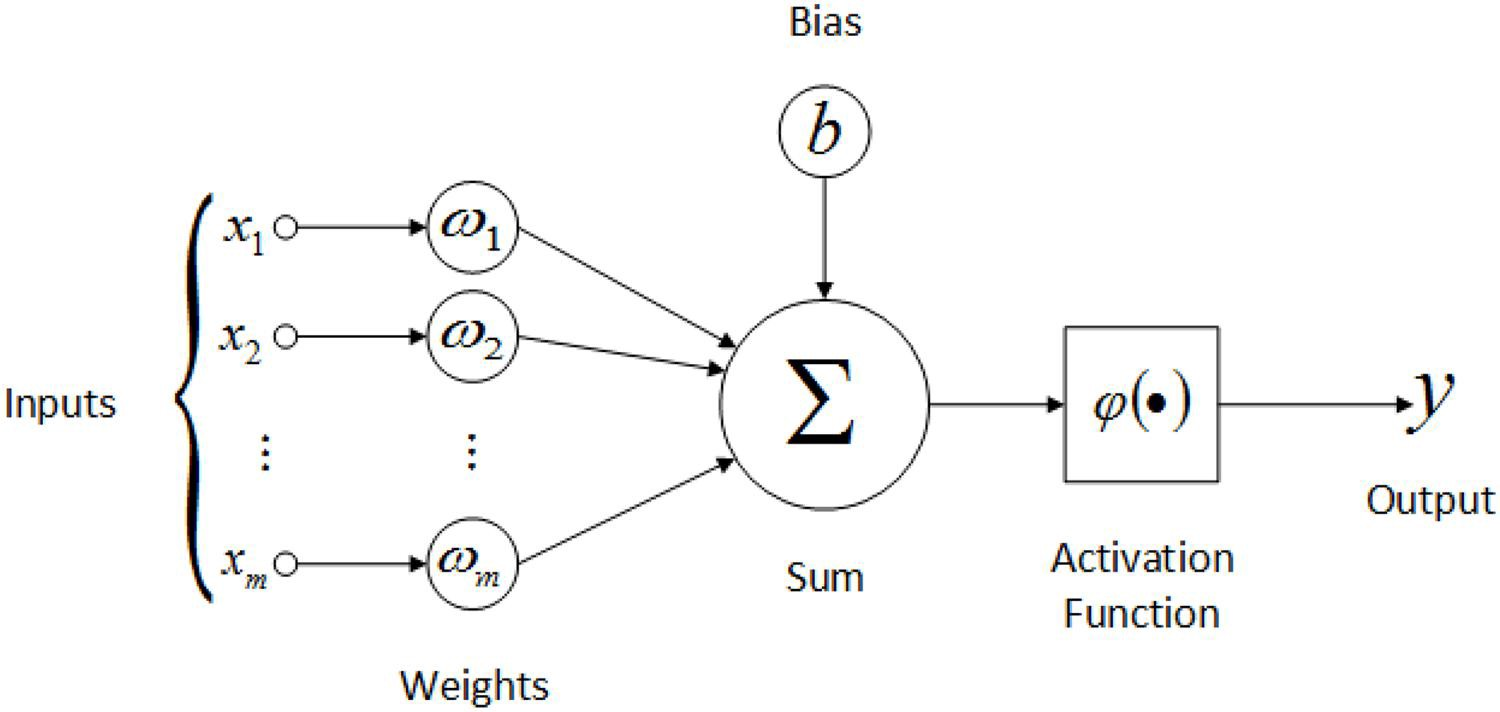
\includegraphics[scale=0.25]{figures/artificialneuron.jpeg}
\caption{Artificial Neuron}
\end{figure}

The activation function is typically the sigmoid function, a hyperbolic tangent, 
or a rectified linear unit (ReLU). They must be a non-linear function because
several layers of linear activation functions still yield a linear decision 
boundary. Deep layers of non-linear activations yield complex decision
boundaries.

\section{Notations}
\begin{itemize}
    \item $a_i^{(j)}$ - Activation of unit $i$ in layer $j$ (the output of the node)
    \item $\theta^{(j)}$ - Matrix of parameters (controlling the activation from one layer to the next)
    \item $g(\theta^Tx)$ - The activation function
\end{itemize}

\section{Multiclass Classification}
\begin{itemize}
    \item Given $N$ classes:
    \begin{itemize}
        \item Build a neural network with $N$ output units
        \item Use one-hot encoding to encode the output as an array of $N-1$ zeros and one $1$.
    \end{itemize}
\end{itemize}

\section{Cost function for Neural Networks}
The cost function can generate $k$ outputs, meaning that the sigmoid function (or any other cost functions) returns a $k$ dimensional vector.

The cost function is combined by two parts.

\bigskip

The first part finds the mean of the sum of each training sample $m$, over the sum of each class $k$. All classes has a "one-vs-all" comparison. This gives the following expression:

\[
    -\frac{1}{m}\left[\sum_{i=1}^m\sum_{k=1}^Ky_k^{(i)} \log\left(h_\Theta(x^{(i)})\right)_k+(1-y_k^{(i)}) \log\left(1-(h_\Theta(x^{(i)}))_k\right)\right]
\]

The second part is the regularization term. In this part, we sum all layers $L-1$, over all units in each layer $s_t$, over all the input layers $j$:

\[
    \frac{\lambda}{2m}\sum_{l=1}^{L-1}\sum_{i=1}^{s_t}\sum_{j=1}^{s_l+1}(\Theta_{ji}^{(l)})^2
\]

\section{Learn this better...}

% 31.30

% \bigskip
% \begin{figure}[H]
% \centering
% \includegraphics[scale=0.5]{figures/}
% \caption{}
% \end{figure}

% \begin{theo}[]{theo:theo}
% \label{eq:}
% \[
% a
% \]
% \end{theo}
%
% \section{}